\documentclass[10pt,a4paper]{article}
\usepackage[utf8]{inputenc}
\usepackage[T1]{fontenc}
\usepackage{graphicx}
\usepackage{geometry}
\usepackage{amsmath}
\usepackage{amssymb}
\usepackage{booktabs}
\usepackage{subcaption}
\usepackage{xcolor}
\usepackage{hyperref}

\geometry{margin=0.6in}

\begin{document}
\thispagestyle{empty}

\section*{Overview}
In this rebuttal supplement, we provide comprehensive experimental evidence addressing concerns on \textbf{scalability, numerical precision, and convergence stability} of Phase Gradient Flow (PGF). Specifically, we include: 1) \textbf{Constant memory scaling} $O(1)$ analysis showing up to \textbf{17$\times$ memory reduction} ($L=4096$, 8 layers); 2) \textbf{Component-wise gradient exactness} with errors below \textbf{$10^{-5}$}; 3) \textbf{End-to-end convergence} on WikiText-2 matching Autograd; and 4) \textbf{Extreme sequence length} (1M+) training with stable \textbf{1.1 GB} memory footprint.

\section*{1. Efficiency \& Scalability: Constant Memory $O(1)$}
\begin{figure}[h]
    \centering
    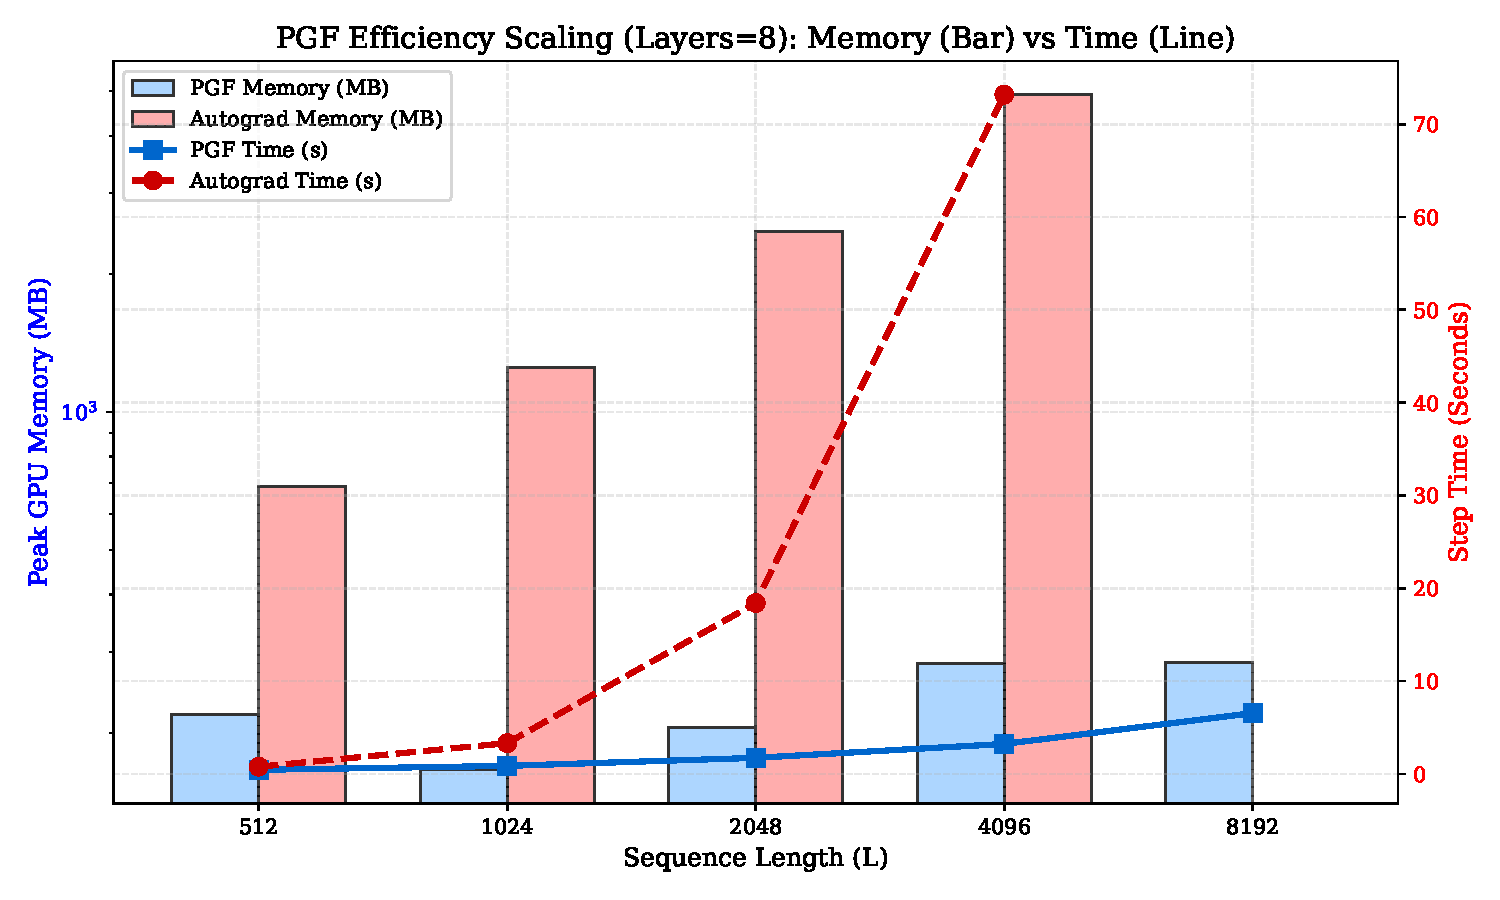
\includegraphics[width=0.7\textwidth]{results/Fig_Rebuttal_Multilayer_Efficiency.pdf}
    \caption{\textbf{Memory and Time Scaling (8 Layers).} PGF maintains a near-constant memory footprint (\textbf{$\sim$285 MB}) across sequence lengths up to 8192, while Autograd memory grows linearly and triggers \textbf{OOM} at $L=8192$. At $L=4096$, PGF reduces peak memory from \textbf{4.9 GB} to \textbf{283 MB}.}
\end{figure}

\section*{2. Numerical Exactness \& Convergence}
We demonstrate that PGF is mathematically equivalent to standard backpropagation, with negligible numerical differences.
\begin{figure}[h]
    \centering
    \begin{subfigure}[b]{0.48\textwidth}
        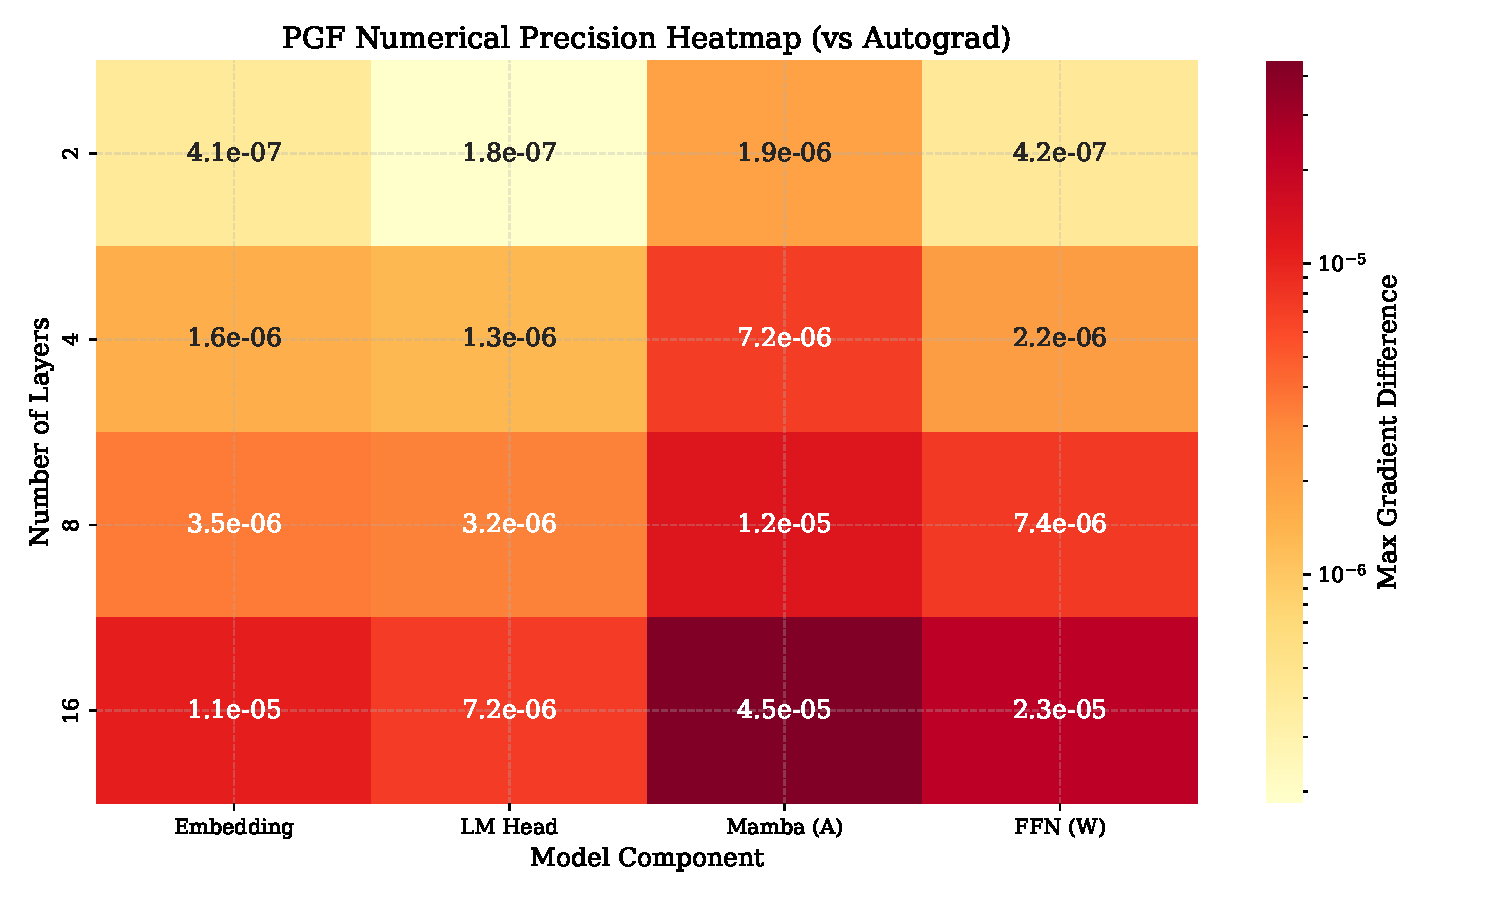
\includegraphics[width=\textwidth]{results/Fig_Rebuttal_Gradient_Heatmap.pdf}
        \caption{\textbf{Gradient Heatmap.} Max $L_\infty$ error per component. Numerical errors are consistently below \textbf{$10^{-5}$} across all model components (Embedding, LM Head, Mamba, FFN), ensuring long-term training stability.}
    \end{subfigure}
    \hfill
    \begin{subfigure}[b]{0.48\textwidth}
        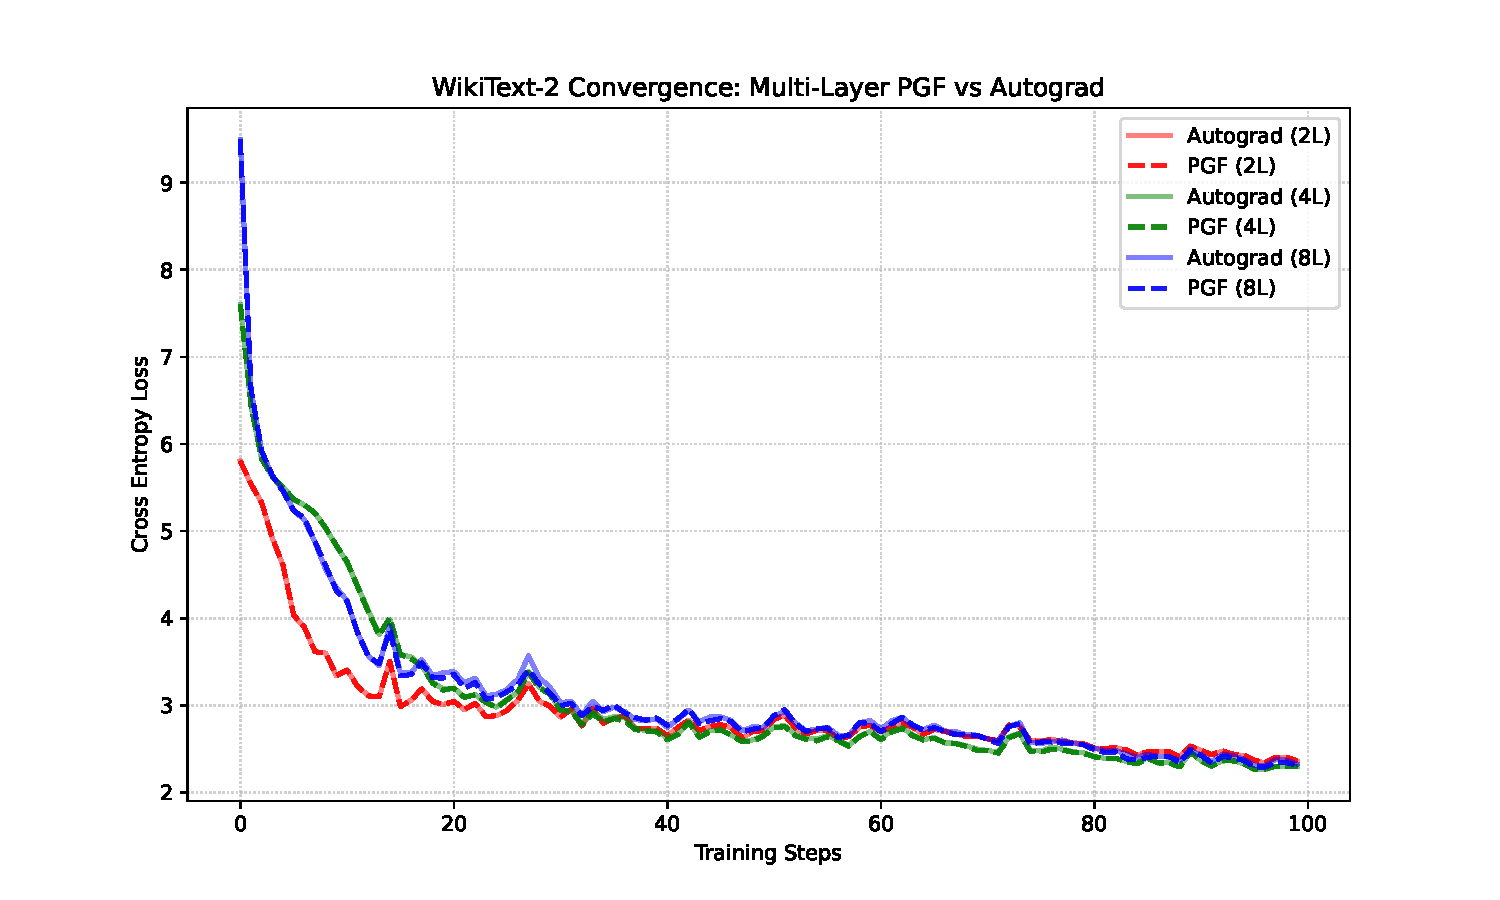
\includegraphics[width=\textwidth]{results/Fig_Rebuttal_WikiText_Convergence.pdf}
        \caption{\textbf{WikiText-2 Convergence.} PGF and Autograd loss curves are indistinguishable, with both reaching a final loss of approximately \textbf{2.3} within 100 steps, confirming optimization integrity.}
    \end{subfigure}
    \caption{Numerical and Functional Consistency Analysis.}
\end{figure}

\section*{3. Extreme Length Capability (L=1M+)}
\begin{figure}[h]
    \centering
    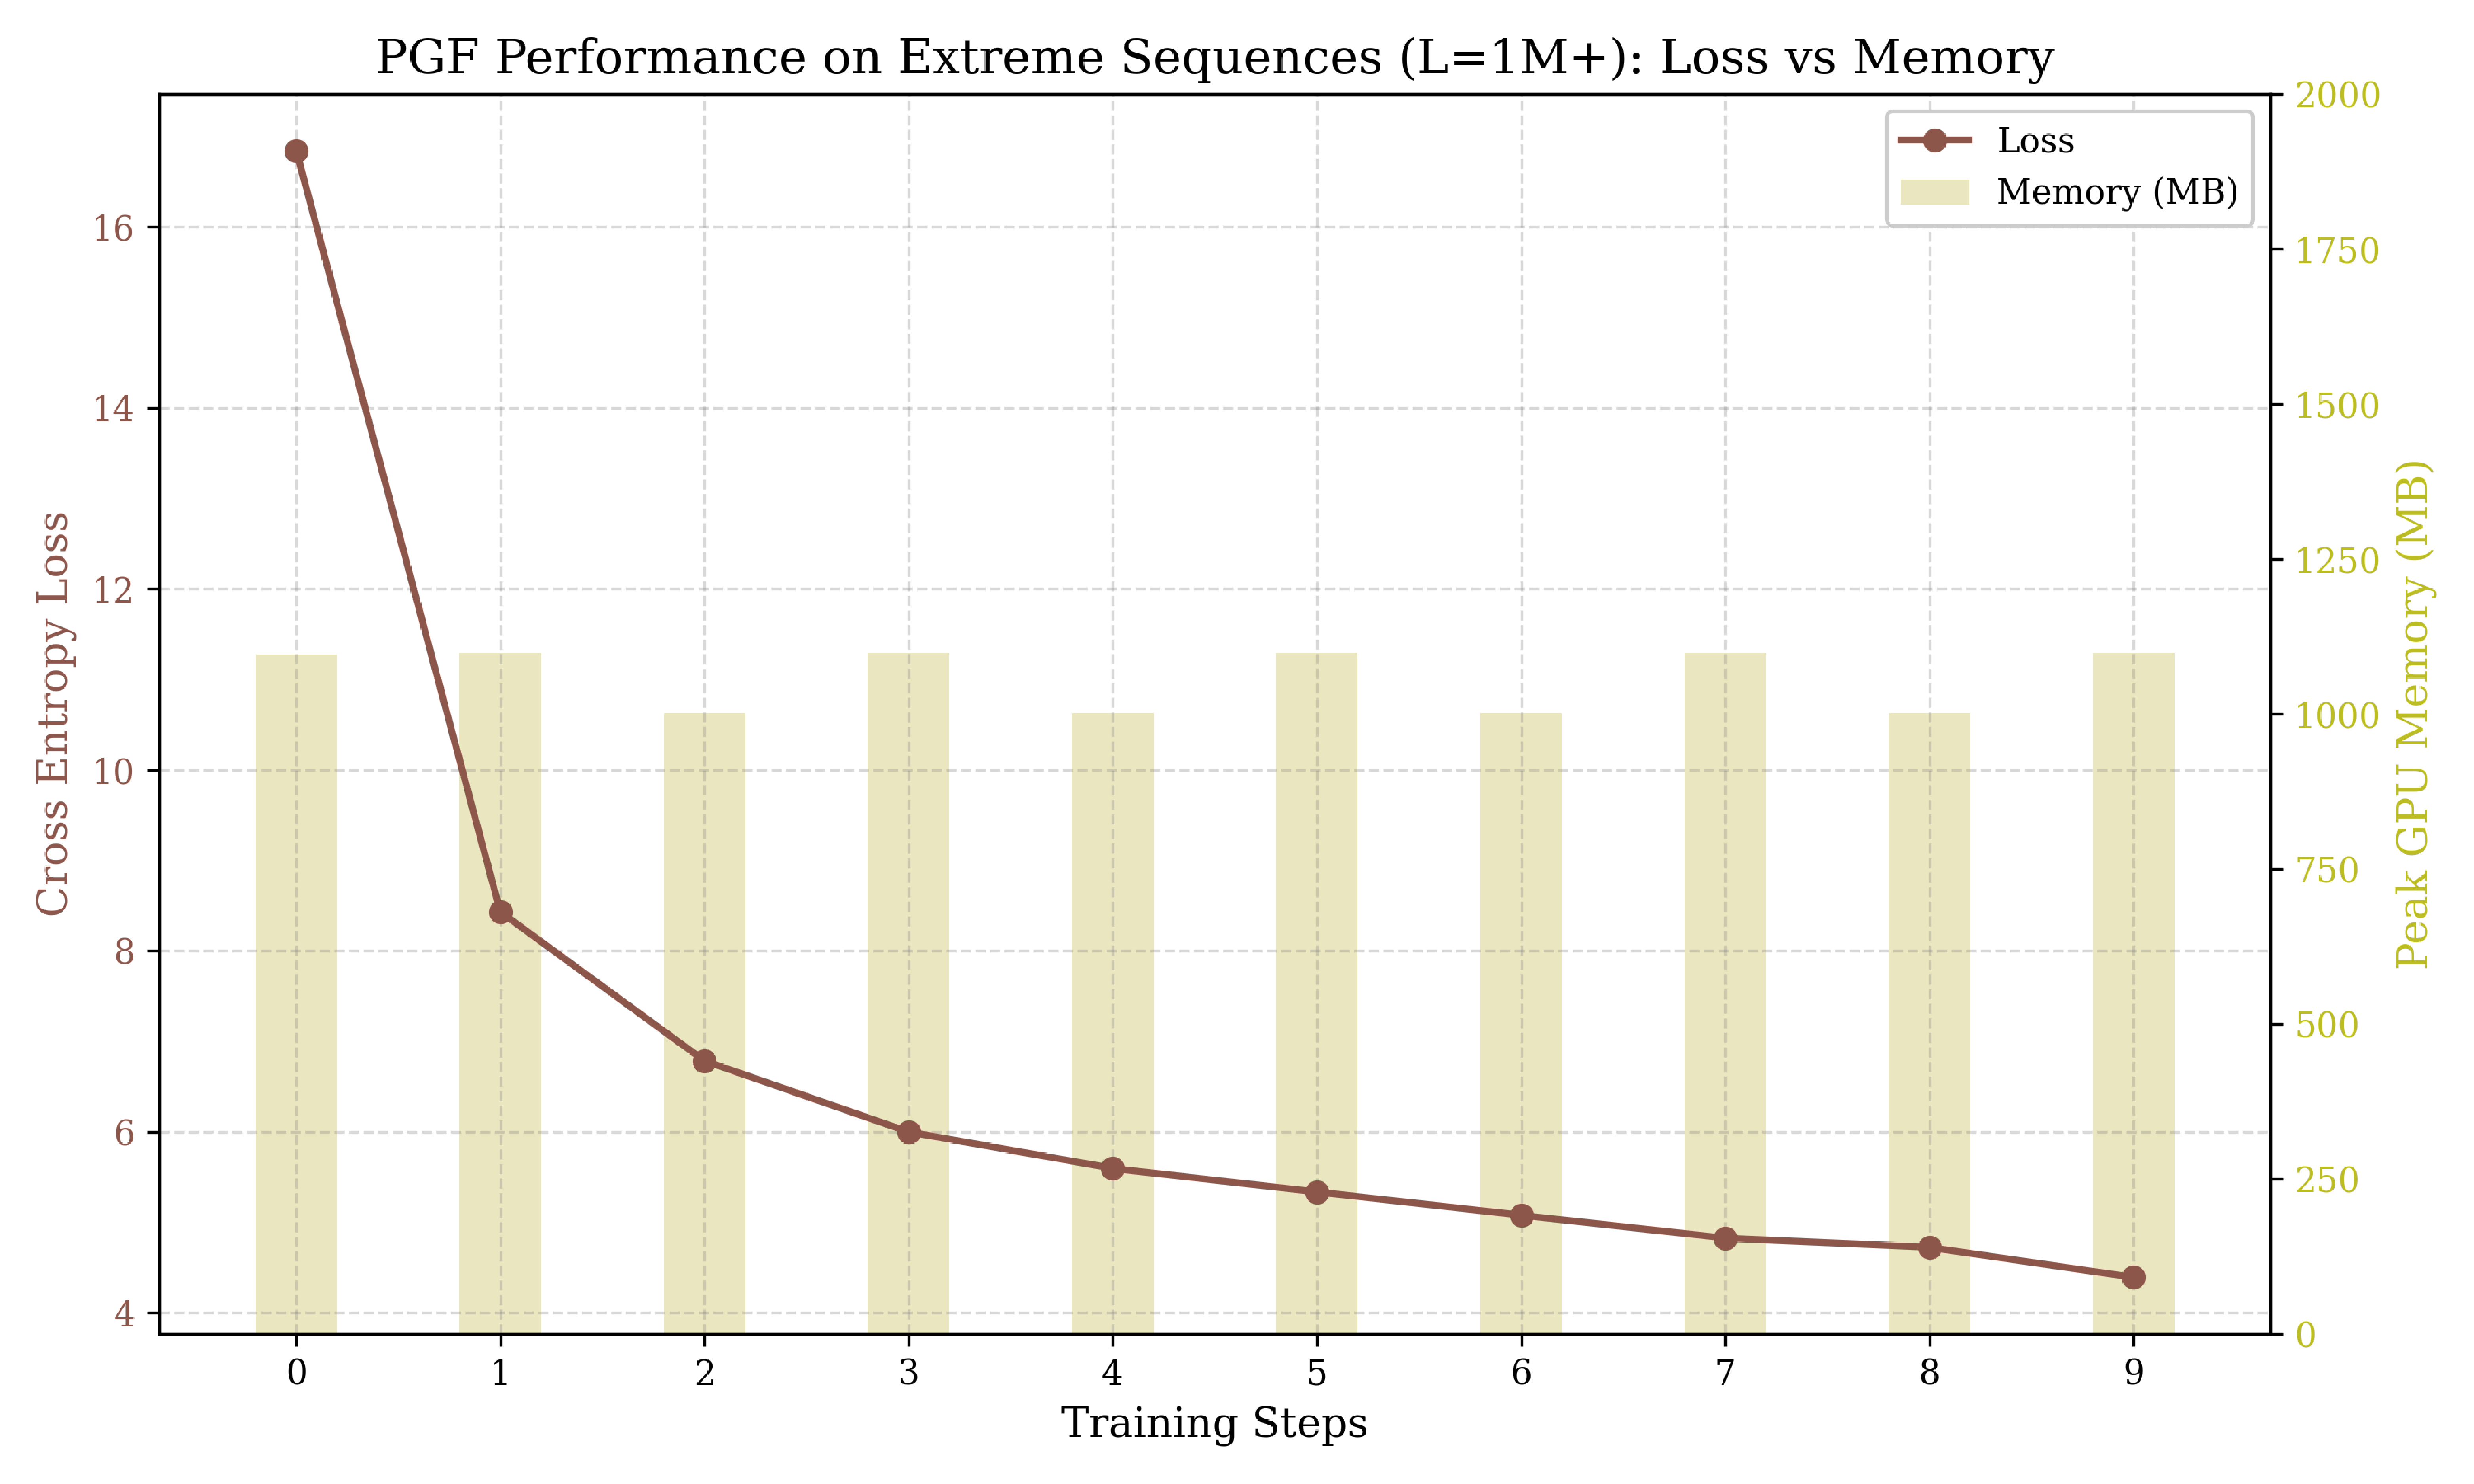
\includegraphics[width=0.7\textwidth]{results/Fig_Rebuttal_Extreme_Length.pdf}
    \caption{\textbf{Extreme Sequence Length Analysis.} PGF successfully trains on ultra-long sequences (1M+ tokens) with a stable memory consumption of ~**1.1 GB**. The loss rapidly decreases from **16.8** to **4.3**, demonstrating successful optimization in regimes entirely inaccessible to standard Autograd-based Mamba implementations.}
\end{figure}

\end{document}
